\documentclass[conference]{IEEEtran}
\usepackage{graphicx}
\usepackage{amsmath}
\usepackage{booktabs}
\usepackage{array}
\usepackage[hidelinks]{hyperref}
\usepackage{balance}
\usepackage{stfloats}

\graphicspath{{../figures/}}

\newcommand{\ugm}{$\mu$g/m$^3$}
\hyphenation{LightGBM}

\setlength{\textfloatsep}{5pt plus 2pt minus 2pt}
\setlength{\dbltextfloatsep}{5pt plus 2pt minus 2pt}
\AtBeginDocument{%
\setlength{\abovedisplayskip}{4pt plus 2pt minus 2pt}%
\setlength{\belowdisplayskip}{4pt plus 2pt minus 2pt}}

\begin{document}

\title{Exact Concept-Grouped SHAP Explanations of a Deployed Real-Time
PM2.5 Ensemble for Texas Census Tracts}

\author{
\IEEEauthorblockN{Saketh Chebrolu}
\IEEEauthorblockA{St. Mark's School of Texas\\
Dallas, TX, USA\\
chebrolusaketh@gmail.com}
\and
\IEEEauthorblockN{Nathan Tan}
\IEEEauthorblockA{St. Mark's School of Texas\\
Dallas, TX, USA\\
nathantan2027@gmail.com}
\and
\IEEEauthorblockN{Yifeng Wang}
\IEEEauthorblockA{School of Civil and Environmental Engineering\\
Georgia Institute of Technology\\
Atlanta, GA, USA\\
ywang3627@gatech.edu}
}

\maketitle

\begin{abstract}
Fine particulate matter (PM2.5) is a leading environmental health risk,
yet regulatory monitors are too sparse to resolve the concentration
gradients that determine neighborhood-scale exposure, and the machine
learning models that fill this gap are consulted operationally although
aggregate skill metrics reveal nothing about where or why they fail. This
paper presents the explanation layer of a publicly deployed system that
maps 24-hour PM2.5 across all 6,896 Texas census tracts on a 30-minute
cycle, fusing 310 quality-screened PurpleAir sensors with
meteorological, wildfire-smoke, and atmospheric-composition data; the
deployed convex tree ensemble over 30 features attains a
leave-one-sensor-out coefficient of determination of 0.71. Blending
per-model TreeExplainer attributions with the deployment weights
reconstructs every pre-clipping prediction, with audited maximum error
below 0.000007 micrograms per cubic meter, and an exhaustive partition of
the features into five concept groups renders each prediction in
physical units. Attribution identifies the system as a
spatial nowcaster: same-day neighboring sensors contribute 4.82
micrograms per cubic meter of mean absolute attribution, against 0.47 for
geography, 0.25 for meteorology, and 0.09 for the dedicated smoke tier.
Removing all eight demographic and source-proximity inputs cost no
measurable accuracy, yet the same neighbor features structurally
suppress hyper-local events: across 46
training episodes above 40 micrograms per cubic meter in which every
neighbor mean was below 5, the regional term was negative in all 46 and
no prediction exceeded 8.5. Exact explanations convert a validated black
box into an operational diagnostic that identifies not only what the map
resolves but where it cannot.
\end{abstract}

\begin{IEEEkeywords}
explainable artificial intelligence, SHAP, air quality, PM2.5, low-cost
sensors, ensemble learning, environmental monitoring
\end{IEEEkeywords}

\section{Introduction}
Regulatory PM2.5 monitoring is sparse relative to the spatial
variability of urban exposure. Low-cost networks such as PurpleAir report
fine particulate matter (PM2.5) at neighborhood scale and minute cadence,
and corrected versions of their data feed public tools such as the
AirNow Fire and Smoke Map \cite{barkjohn2021}. Sensor placement is itself
uneven across income groups \cite{desouza2021}; for many communities,
models interpolating between sensors are the sole source of air quality
information.

Such models are evaluated almost exclusively by aggregate accuracy,
which can conceal behavior their operators would not endorse; when
outputs color a public map or guide monitor placement, unexamined
behavior is an operational risk. Shapley additive explanation (SHAP)
methods \cite{lundberg2017, lundberg2020} have made attribution
tractable for tree models, and environmental applications such as
flood-susceptibility mapping have begun to adopt them \cite{choubin2025}.
Published explanations, however, almost invariably concern research
models; deployed systems remain unexamined.

This paper provides an exact explanation of one deployed system: a live
web platform that predicts PM2.5 for every Texas census tract from
PurpleAir sensors and public data streams. The contributions are
threefold: (1) an exact explanation layer for the
deployed convex tree ensemble, in which per-model TreeExplainer
attributions blended with the deployment weights reconstruct every
pre-clipping output to machine precision, and a partition of the 30
features into five concept groups expresses each prediction in physical
units; (2) a characterization of the deployed model as a spatial
nowcaster dominated, to a degree aggregate metrics do not reveal, by
same-day readings from neighboring sensors; and (3) an
explanation-driven failure analysis demonstrating that the neighbor
features responsible for the model's accuracy actively suppress its
predictions during hyper-local pollution events, a structural limitation
that motivates targeted sensor placement rather than model tuning.

\section{The Deployed System}
\label{sec:system}
\subsection{Platform}
The platform serves a public, bilingual web map of model-estimated
24-hour PM2.5 for all 6,896 Texas census tracts, public since April 2026.
The backend retrieves live PurpleAir readings, cached for 15 minutes,
recomputes the full feature set, runs the ensemble for every tract, and
caches predictions for 30 minutes. A served value estimates a tract's
daily-mean-equivalent PM2.5 under current conditions; the training
pipeline is reproduced at serving time, so sub-daily dynamics enter only
through the inputs. The
tract color scale breaks at 9~\ugm{}, the 2024 annual PM2.5 standard
\cite{epa2024naaqs}, as a fixed reference for the 24-hour map. A second view proposes future sensor placements, to which
Section~\ref{sec:discussion} returns.

\subsection{Training data and features}
The training target is the daily mean of the raw PurpleAir ATM-channel
PM2.5 concentration. Readings are restricted to 0 to 200~\ugm{} and
cleaned per sensor with a robust z-score rule on median absolute
deviation; sensors with fewer than 60 valid days, near-constant output,
or medians indicating indoor placement are excluded. The corpus comprises
285,798 daily readings from 310 outdoor Texas sensors between January
2021 and May 2026. Sensors in border states contribute
same-day neighbor context but are never training targets. The raw ATM
channel is retained, rather than corrected \cite{barkjohn2021}, so that
training targets and live inference share semantics;
Section~\ref{sec:discussion} revisits this choice. Days with means above
75~\ugm{} are excluded from training, a decision the explanations
quantify.

Each row carries 30 features (Table~\ref{tab:groups}): daily weather from
Open-Meteo \cite{zippenfenig}; same-day neighbor statistics (mean and
count of other sensors within 25, 50, and 100~km, plus dispersion at
50~km, computed with a haversine BallTree); an ordinal smoke tier from
NOAA Hazard Mapping System (HMS) analyst polygons \cite{brey2018};
aerosol optical depth and surface PM2.5 from the Copernicus Atmosphere
Monitoring Service (CAMS) \cite{peuch2022}; location and distance
covariates; and calendar encodings.

No EPA EJScreen variable is a model input. An earlier deployment carried
eight (four demographic and four source-proximity) accounting for 12.1\%
of blended attribution \cite{ejscreen}; all eight were removed before
this study, because a model used to characterize exposure disparities
must not receive those groups as predictors, or any disparity it
reproduces is partly an artifact of its own inputs. Removal cost was
measured on frozen sensor-grouped folds with the blend held fixed:
dropping the four demographic features changes $\Delta R^2 = 0.0022$
(95\% CI $[-0.0031,+0.0083]$) and dropping all eight $-0.0005$
($[-0.0070,+0.0066]$); both intervals contain zero, and the negative
sign indicates the smaller model scored marginally higher.

\subsection{Ensemble and validation}
Four regressors are trained: a random forest \cite{breiman2001}, LightGBM
\cite{ke2017}, XGBoost \cite{chen2016}, and CatBoost
\cite{prokhorenkova2018}. Validation is leave-one-sensor-out (LOSO): each
of the 310 sensors is held out in turn, models are refit on the
remainder, and the neighbor features of every training row are recomputed
with the held-out sensor removed, closing a same-day leakage path that
random splits cannot detect. Spatially naive
cross-validation is known to overstate the skill of models of this class
\cite{meyer2022}; under random 80/20 splitting this ensemble scores
$R^2=0.80$, which LOSO deflates to 0.71. LightGBM and XGBoost use Huber
and pseudo-Huber objectives respectively: PM2.5 is heavy-tailed, and
squared error lets a few smoke and dust days dominate the fit.

Blend weights are a simplex-constrained convex combination fit on the
LOSO out-of-fold predictions and selected by a grouped cross-fit over
sensors. The deployed weights are 0.7935 (random forest), 0.1363
(CatBoost), 0.0702 (LightGBM), and exactly zero for XGBoost, giving LOSO
$R^2=0.7134$ against 0.7084 for an equal-weight blend and 0.7090 for an
inverse-MSE baseline. The deployed configuration scores RMSE 4.21~\ugm{}
and MAE 2.61~\ugm{}. The random forest alone reaches 0.7138: the leading
candidates are tied at this resolution, and the deployment is a nearly
single-model instance of the convex blends the method covers; the blend
is explained because the blend is deployed. Live inference imputes
unavailable features with training medians.

\begin{table}[!t]
\caption{The five concept groups partitioning the 30 model features
(group sizes in parentheses).}
\label{tab:groups}
\centering
\footnotesize
\begin{tabular}{>{\raggedright\arraybackslash}p{0.30\columnwidth}>{\raggedright\arraybackslash}p{0.58\columnwidth}}
\toprule
Group & Features \\
\midrule
Regional PM signal (9) & neighbor PM2.5 mean and count at 25, 50, 100 km;
dispersion at 50 km; CAMS AOD; CAMS PM2.5 \\
Wildfire smoke (1) & HMS smoke tier (none/light/medium/heavy) \\
Meteorology (7) & temperature, humidity, pressure, wind speed,
precipitation, two interaction terms \\
Geography (4) & latitude, longitude, distance to coast, distance to
nearest sensor \\
Season and calendar (9) & month, weekday, day of year, and their
sine/cosine encodings \\
\bottomrule
\end{tabular}
\end{table}

\section{Exact Ensemble Explanations}
\subsection{Blending per-model attributions}
The deployed prediction for features $x$ is
$f(x)=\max\bigl(0,\sum_m w_m f_m(x)\bigr)$ over the three models with
$w_m>0$. TreeExplainer \cite{lundberg2020} decomposes each tree model
exactly as $f_m(x)=b_m+\sum_j \phi^m_j(x)$. Attributions are additive, so
\begin{equation}
\sum_m w_m f_m(x) = b + \sum_j \phi_j(x),
\label{eq:blend}
\end{equation}
where $b=\sum_m w_m b_m$ and $\phi_j(x)=\sum_m w_m \phi^m_j(x)$. The
result is an additive decomposition of the pre-clipping ensemble output,
computed without sampling or surrogate models. The algebra follows
immediately from the additivity of SHAP attributions \cite{lundberg2017};
its value lies in applying it to the ensemble a public platform serves. Exactness denotes local accuracy, faithful reconstruction of this
model's output, not axiomatic Shapley values under an interventional
distribution: TreeExplainer (SHAP 0.50.0) runs in tree-path-dependent
mode, conditioning on the training distribution through tree cover
counts, so credit assignment among correlated features differs from
interventional variants. The audit of Eq.~\eqref{eq:blend} executes
wherever rows are explained. Over the 6,000-row global sample the maximum
absolute reconstruction error is below $7\times10^{-6}$~\ugm{}; the
residual reflects float32 caching, and
direct float64 explanation of individual rows reconstructs to
$5\times10^{-14}$~\ugm{}. The serving layer applies only a final clip at
zero, which never binds on the sampled predictions (minimum raw output
$+0.4$~\ugm{}).

\subsection{Concept groups}
Individual attributions for 30 features are exact but not interpretable
by a public audience. The features are therefore partitioned into the
five concept groups of Table~\ref{tab:groups}, and group sums
$\Phi_G(x)=\sum_{j\in G}\phi_j(x)$ are reported, the summation form of
grouped Shapley explanation \cite{jullum2021}; the contribution is the
ontology, not the operation. Because the partition is
exhaustive and disjoint, $b+\sum_G \Phi_G(x)$ reconstructs the prediction
exactly, and runtime validation asserts the partition against the
deployed feature list. A group's global importance, the mean absolute
summed contribution, falls below the sum of member importances when
members cancel.

\subsection{Analysis protocol}
Global structure is computed over a uniform 6,000-row sample of the
training frame (seed 42). Feature response is analyzed with dependence
scatters, 12-quantile binned medians, and Spearman rank correlations
between feature value and attribution, with bootstrap intervals clustered
by sensor. Because the sample contains only five heavy-smoke rows,
tier-level smoke statistics are recomputed exactly over all 431
heavy-tier corpus rows and a 2,500-row medium-tier sample,
with 2,000-resample percentile-bootstrap 95\% confidence intervals
clustered by day, because statewide plumes correlate same-day rows. Two
full days are explained sensor-by-sensor: the strongest smoke day (May
27, 2024) and the cleanest day (April 3, 2024) among days with at least
150 reporting sensors. Local cases follow fixed selection rules: the
highest-reading smoke-day row predicted within 35\% of its observation,
and the worst underprediction above 40~\ugm{}. All pipeline outputs
reproduce byte-identically; every analysis number is regenerated by
verification scripts released with the code.

\begin{figure}[!t]
\centering
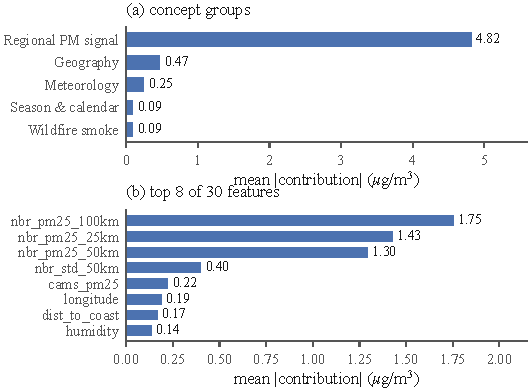
\includegraphics[width=0.88\columnwidth]{fig2_global}
\caption{Global importance over the 6,000-row sample. (a) Mean absolute
concept-group contribution; the regional PM signal exceeds every other
group by an order of magnitude. (b) The top individual features are the
three neighbor means, neighbor dispersion, and CAMS surface PM2.5.}
\label{fig:global}
\end{figure}

\section{Results}
\subsection{The model is a spatial nowcaster}
Fig.~\ref{fig:global} shows global importance. The regional PM signal
group averages 4.82~\ugm{} of absolute contribution per prediction (95\%
CI $[4.71,4.93]$); the next group, geography, averages 0.47~\ugm{}
$[0.41,0.53]$, an order of magnitude smaller, followed by meteorology at
0.25~\ugm{}, season and calendar at 0.091~\ugm{}, and the dedicated smoke
tier last at 0.090~\ugm{}. The three neighbor-mean features are
individually the three most important inputs (1.75, 1.43, and 1.30~\ugm{}
at 100, 25, and 50~km). The ensemble's predictions are, before all else,
spatial averages of what nearby sensors currently report.

The top of the ordering is unambiguous: the regional group's interval is
disjoint from every other, and grouped permutation importance reproduces
the ranking exactly (rank correlation 1.0). The full five-way ranking
survives 65.8\% of 1,000 sensor-clustered resamples, with the instability
confined to the bottom pair: season (0.091) and smoke (0.090) differ by
0.001~\ugm{}, so their order is not resolved.

\begin{figure*}[b]
\centering
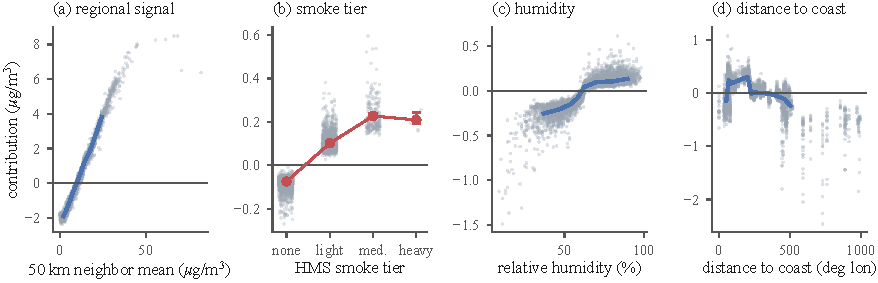
\includegraphics[width=0.92\textwidth]{fig3_dependence}
\caption{Feature dependence on the 6,000-row sample (gray points; blue line
is the 12-quantile binned median). (a) Contribution of the 50 km neighbor
mean is near-linear then flattens above 40~\ugm{}. (b) HMS smoke tier:
red markers are exact means over all 431 heavy-tier rows and 2,500
medium-tier rows with day-clustered bootstrap 95\% intervals; the heavy
tier shows no increase over medium.
(c) Humidity contributes weakly but monotonically, with a threshold near 60\% RH. (d) Distance to
coast trends negative inland, encoding the Gulf moisture gradient and
sensor-network density rather than a causal effect of position.}
\label{fig:dependence}
\end{figure*}

\subsection{Feature response and semantics}
Dependence analysis (Fig.~\ref{fig:dependence}) yields four findings.

\subsubsection{Near-linear regional response} The 50~km neighbor mean
maps onto its attribution almost monotonically (Spearman $\rho=0.993$),
with slope 0.25~\ugm{} per 1~\ugm{} of neighbor mean below 30~\ugm{},
then flattens: over corpus rows, the median contribution is
$+5.78$~\ugm{} for neighbor means between 30 and 40~\ugm{} (2,000 of
4,060 rows sampled) and $+7.39$~\ugm{} (CI $[7.37, 7.43]$, all 860
qualifying rows) above 40~\ugm{}. The flattening is consistent with the
exclusion of training days above 75~\ugm{}: the model has no basis to
extrapolate beyond its training range.

\subsubsection{The smoke tier is nearly redundant} Mean attribution of
the HMS tier, in \ugm{}, is $-0.074$ (none) and $+0.101$ (light) on the
sample, $+0.227$ over 2,500 recomputed medium-tier rows (day-clustered CI
$[0.218, 0.238]$), and $+0.209$ over all 431 heavy-tier rows (CI
$[0.191, 0.243]$; the heavy rows fall on only 31 days). Heavy-tier
attribution shows no increase over medium (difference CI
$[-0.018, 0.041]$~\ugm{}), and the entire tier range is negligible
against a LOSO RMSE near 4.2~\ugm{}. Only 431 of 285,798 training rows
(0.15\%) carry the heavy tier, and on those rows mean observed PM2.5 is
lower than on medium-tier rows (11.6 versus 16.6~\ugm{}): an
analyst-drawn plume overhead does not guarantee surface-level smoke. The
model largely disregards a feature whose evidential value its training
data did not support.

\subsubsection{The disparity survives the exclusion} Correlating tract
predictions (6,896 tracts, 365 days) post hoc against EJScreen
percentiles the model never receives, low income rises monotonically
across quintiles from 8.58 to 9.29~\ugm{} ($\rho=0.16$); percent people
of color is non-monotone, dipping to 8.67 mid-range before reaching 9.38.
The disparity is real but non-uniform and, absent demographic inputs, is
inferred from atmospheric evidence alone.

\subsubsection{Interactions remain within the regional group} SHAP
interaction values (a 400-row subsample, seed 42; random forest and
CatBoost blended with renormalized weights covering 93\% of the deployed
ensemble, LightGBM omitted because its interaction runtime exceeded
budget) rank the six leading pairs entirely within the regional signal
group: the three neighbor means interact at 0.48, 0.41, and 0.30~\ugm{}
mean absolute strength, followed by three neighbor-dispersion pairs. The
strongest cross-group pair, humidity with the 100~km neighbor mean, is
weaker at 0.06~\ugm{}. Regional dominance is therefore not an artifact of
additive attribution. Magnitudes are taken \emph{after} the signed blend,
so model disagreement cannot inflate a pair.

\begin{figure}[!b]
\centering
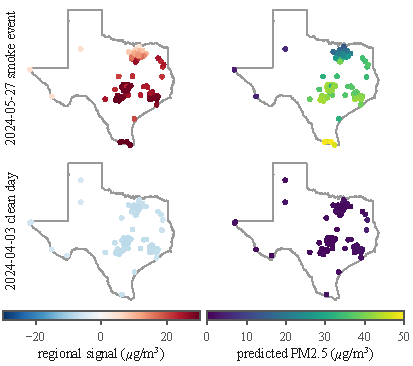
\includegraphics[width=0.87\columnwidth]{fig4_event_maps}
\caption{Every reporting sensor explained on the strongest smoke day
(top, 156 sensors, 98.7\% under a plume) and the cleanest day (bottom, 154
sensors): regional-signal contribution (left) and predicted PM2.5 (right).
The event is carried almost entirely by the regional signal
($+24.3$~\ugm{} statewide mean) while the smoke tier peaks at
$+0.64$~\ugm{} anywhere in the state.}
\label{fig:maps}
\end{figure}

\subsection{Contrasting days, one mechanism}
On May 27, 2024 (Fig.~\ref{fig:maps}), with 98.7\% of sensors under an
analyst-drawn plume and a statewide mean reading of 37.0~\ugm{}, the
model predicted a mean of 36.0~\ugm{}, of which the regional signal group
contributed $+24.3$~\ugm{} on average; the smoke tier's mean contribution
that day was $+0.4$~\ugm{}. On April 3, 2024 (statewide mean
1.03~\ugm{}), the regional group lowered predictions by 7.6~\ugm{} on
average from the 9.65~\ugm{} baseline. Smoke information reaches the
model through the neighbor network rather than the smoke feature: both
days instantiate the same nowcasting mechanism.

\subsection{Case analysis: a detection and a miss}
Fig.~\ref{fig:cases} decomposes two individual predictions. On the smoke
day, sensor 217461 read 71.1~\ugm{} and the model predicted 49.8~\ugm{},
with $+34.6$~\ugm{} from the regional signal and $+0.64$~\ugm{} from the
smoke tier; even this detection underpredicts, consistent with the capped
training range and the saturating neighbor response. On November 19,
2024, sensor 242357 read 75.0~\ugm{}, at the retention boundary itself,
while every neighbor mean sat below 1.8~\ugm{}; the model predicted
5.1~\ugm{}. The explanation is direct: the regional group
contributed $-5.9$~\ugm{}, with the 100~km neighbor mean alone at
$-2.2$~\ugm{}. The case is not isolated: 46 corpus rows read at least
40~\ugm{} with every neighbor mean below 5~\ugm{}; the regional group is
negative on all 46 (mean $-4.9$~\ugm{}), and the highest prediction among
them is 8.5~\ugm{} against a mean observation of 54.1~\ugm{}. Rows above
75~\ugm{} were excluded before training (241 pre-cap), so these figures
lower-bound the blind spot. The features that make the model accurate on
regional events actively vote against hyper-local ones; no reweighting of
the same features can recover what the network does not observe.

\begin{figure}[!b]
\centering
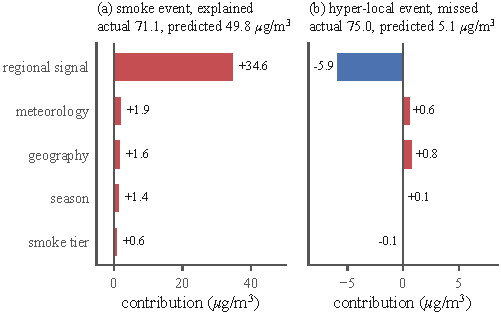
\includegraphics[width=0.87\columnwidth]{fig5_cases}
\caption{Exact concept-group decomposition of two predictions. (a) A
detected smoke event is carried by the regional signal; the smoke tier
adds $+0.6$~\ugm{}. (b) The worst miss in the corpus: neighbors observed
nothing, and the regional signal suppresses the prediction below the
baseline.}
\label{fig:cases}
\end{figure}

\section{Discussion}
\label{sec:discussion}

\subsection{Model development} The smoke tier warrants replacement rather
than retuning: candidate representations include plume density, smoke
age, and lagged fire radiative power. The saturating neighbor response
follows from the 75~\ugm{} training cap; raising the cap is a measurable
next experiment.

\subsection{Network operation} The miss case converts an error metric
into a map, subject to one caution: sign alone cannot separate clean
surroundings from unobserved ones (the clean day's statewide mean
regional contribution, $-7.6$~\ugm{}, is as negative as El Paso's annual
$-6.8$~\ugm{}). Sparsity separates them: the El Paso sensor averages 0.8
same-day neighbors within 50~km against a statewide 27, and its regional
contribution averages $-6.8$~\ugm{} against East Texas's $+1.34$~\ugm{}
(up to $+9.4$). Persistently negative regional means in sparse
neighborhoods mark locations where predictions rest on remote evidence
(distance to the nearest sensor reaches 164~km), and these are where the
platform's placement optimizer should allocate new sensors; the
explanation layer supplies this prioritization directly.

\subsection{Communicating attributions} SHAP explains the model, not the
atmosphere. Distance to coast and longitude are the clearest example:
both carry real signal, but they encode sensor-network position and the
Gulf moisture gradient, not a causal effect of coordinates. Public-facing deployment of these
explanations requires the concept-group framing and an explicit
correlational disclaimer as defaults, not footnotes. Carrying no
demographic input (Section~\ref{sec:system}) removes the most severe
misreading risk but does not make the remaining attributions causal.

\subsection{Limitations} The target is the uncorrected ATM channel, so
absolute levels are not comparable to regulatory monitors without a
correction such as that of Barkjohn et al. \cite{barkjohn2021}, and the
explanations inherit whatever bias that channel carries. Days above
75~\ugm{} are absent from training, so extreme-event behavior describes a
model that never observed the worst days, and the failure analysis
lower-bounds the blind spot. LOSO $R^2$ characterizes held-out sensor
locations; accuracy at unsensed tracts is unquantified, and the miss case
indicates it degrades precisely there. Every attribution is conditioned
on a network whose placement is itself demographically uneven
\cite{desouza2021}: the regional-signal group is strongest where sensors
are dense, so the explanations describe an unevenly observed state. Tree-path-dependent attribution
spreads credit among correlated features, so within-group rankings are
less certain than group totals. Explanation statistics describe the
training frame, not the serving distribution. The findings describe one
model, one state, and five years; the method applies to any convex blend
of tree models.

\balance
\section{Conclusion}
This work converted a deployed, accuracy-validated PM2.5 mapping system
into one whose every prediction can be read: an exact blend of per-model
TreeExplainer attributions, folded into five concept groups, reconstructs
each output to machine precision. The resulting characterization is in
part unfavorable: the model is a spatial nowcaster that largely
disregards its smoke tier, uses geography as a proxy for network density,
and cannot detect events its network does not observe. None of these
properties is visible in $R^2$, and all of them bear on how the tool
should be used, improved, and communicated. Explaining 6,000 predictions
requires under six minutes on a desktop CPU, and a single prediction a
fraction of a second; integrating exact, narrated explanations into the
live platform is the immediate next step.

\bibliographystyle{IEEEtran}
\bibliography{../references}

\end{document}
